\chapter{Súčasný stav}

\label{kap:vychodisko}

Kapitola predstavuje roboty Otto a Mokrarosa, na ktorých riadenie sa v práci zameriavame. Uvádzame možnosti a obmedzenia plynúce z aktuálnej implementácie ich riadiacich programov, ako aj z ich fyzickej konštrukcie. Súčasťou je prehľad podobných riešení, ktorými sa možno pri práci inšpirovať.

% ===
% === Robot Otto a Mokrarosa
% ===
\section{Robot Otto a Mokrarosa}
Cieľom práce nie je stavba robota, zameriavame sa na riadenie existujúcich robotov, najmä modelu Otto a Mokrarosa. Tieto roboty boli použité vo výučbe v rámci denných táborov v bratislavskom Fablabe a tiež v tábore IT Akadémie. Sú teda testované v praxi, poznáme ich nedostatky ale i potenciál, ktorý máme v pláne rozvíjať. Na prvý pohľad možno badať podobu danú výrobným procesom, nakoľko oba roboty sú tlačené 3D tlačiarňou, rozmermi sú kompaktné, konštrukciou relatívne jednoduché. Modularita konštrukcie sľubuje rozšíriteľnosť v mnohých smeroch, roboty sú principiálne podobné no majú aj svoje špecifiká. Treba zdôrazniť, že ich primárnym určením nie je zdolávanie prekážok alebo fyzická manipulácia s nejakými predmetmi, aj keď nie je vylúčená. Primárne sa jedná o edukačné, demonštračné zariadenia.

% Arduino
\subsection{Riadiaca jednotka --- Arduino Nano}
Hlavným komponentom ktorý využívajú oba roboty je riadiaca jednotka --- jednočipový mikropočítač Arduino Nano (resp. Arduino Nano Strong v prípade robota Mokrarosa). Verziu Nano môžete vidieť na obrázku \ref{obr:arduino}. Arduino je open--source platforma používaná vo viacerých projektoch na riadnie rôznych zariadení, existuje viacero verzii, ktoré sa líšia výkonom i funkciami \cite{ArduinoConcept}. V našom prípade mikropočítač riadi všetky funkcie robota, teda napríklad vysiela riadiace impulzy pre ovládanie pohybu servomotorov alebo vysielanie zvukových signálov. Taktiež je zodpovedný za komunikáciu so senzormi a je ho možné prostredníctvom počítača programovať. Pre účely tejto práce je najdôležitejším parametrom daným použitím tohto komponentu pamäť. Konkrétne Arduino Nano disponuje 32KB flash pamäte (z čoho 2KB využíva bootloader), pamäťou SRAM o veľkosti 2KB a 1KB pamäte typu EEPROM \footnote{Electrically Erasable Programmable Read--Only Memory --- elektricky zmazateľná pamäť ROM} \cite{ArduinoNanoSpecification}. Je teda zrejmé, že je žiaduce s pamäťou pri implementácii riadiacich programov pokiaľ možno čo najviac šetriť. Komunikácia s mikropočítačom prebieha pripojeným USB káblom, ktorým je možné nahrať do pamäte riadiaci program. Po spustení je možné s programom komunikovať buď to prostredníctvom už spomínaného rozhrania USB, alebo bezdrôtovo, čo umožňuje integrované rozhranie BlueTooth. K dispozícii sú tiež analógové a digitálne piny, ktoré možno softvérovo riadiť. Použiteľné sú ako vstup alebo výstup, pomocou nich je Arduino schopné ovládať motory a načítavať hodnoty zo senzorov. Na obrázku \ref{obr:arduino} ich možno vidieť na hornej a spodnej časti dosky.

\begin{figure}
\centerline{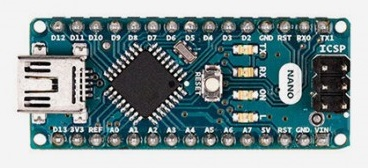
\includegraphics[width=0.4\textwidth]{images/arduino-nano}}
\caption[Riadiaca jednotka - Arduino Nano]{Riadiaca jednotka robota - Arduino Nano}
\label{obr:arduino}
\end{figure}

\subsubsection{Programovanie mikropočítača Arduino}
Programovací jazyk Arduino je založený na jazyku C++, sú v ňom však navyše dostupné rôzne funkcie a knižnice umožňujúce ovládanie špecifických prvkov mikropočítača, najmä riadenie periférii, senzorov a motorov pomocou pinov \cite{ArduinoLanguage}. Periférie je teda možné jednoducho ovládať volaním príslušnej funkcie. K dispozícii je tiež voľne dostupný Arduino Software (IDE), v ktorom možno v textovom editore písať program, jedným kliknutím ho kompilovať, po pripojení USB kábla načítať do pamäte Arduina a spustiť. Program tvoria dve hlavné časti, metódy setup a loop. Metóda setup sa vykoná pri spustení programu práve raz, slúži predovšetkým na inicializáciu premenných, prípadne kalibráciu motorov, senzorov, určenie parametrov pinov a podobne. Metóda loop je následne vykonávaná v nekonečnom cykle, obsahuje hlavný program. S ohľadom na obmedzenia plynúce z veľkosti dostupnej pamäte je kód písaný v jazyku C++ zvyčajne čo najjednoduchší, s preferenciou jednoduchých štruktúr a pamäťovo úspornejších prvkov jazyka C.

% Riadiaci program
\subsection{Riadiaci program}
Riadiaci program robota je vždy možné vytvoriť priamo ako program pre Arduino popísaný vyššie. V prípade denných táborov bolo ale zvolené iné riešenie, umožňujúce riadiť robota aj bez znalosti C++. Princíp je nasledovný. Riadiaci program napísaný v C++ prijíma počas behu, v časti loop, cez sériový port (pripojenie rozhraním USB alebo bezdrôtovou technológiou BlueTooth) postupnosť znakov, ktoré majú predurčený význam. Znaky rozpoznáva, a interpretuje ako príkazy. Na strane užívateľa je teda riadenie robota vykonávané zadávaním reťazca do znakového terminálu (napríklad prostredníctvom programu Putty v OS Windows). Popísaným spôsobom je možné riadiť robota manuálne ale i vytvárať jednoduché choreografie. Viac o programovaní a ovládaní uvádzame v častiach venovaných samostatným robotom, nakoľko ich možnosti nie sú totožné. Výhodou prístupu je mimo iného fakt, že pri ladení choreografie nie je potrebné zakaždým kompilovať program pre Arduino. Ústredným nedostatkom je na druhú stranu výraznejšie obmedzená dĺžka choreografie, keďže je nutné všetky jej prvky reprezentovať a uchovať v operačnej pamäti.

% Interakcia s prostredím
\subsection{Interakcia s prostredím}
Roboty interagujú s prostredím použitím receptorov, ktorými získavajú údaje z prostredia a efektorov, ktorými prostredie ovplyvňujú. K mikropočítaču Arduino možno pripojiť rôzne periférie. Aktuálna konštrukcia robotov Otto a Mokrarosa zdieľa použitie komponentov servomotor a ultrazvukový senzor.

\subsubsection{Servomotor}
TODO - princíp a možnosti

\subsubsection{Ultrazvukový senzor}
TODO - princíp a možnosti

% Otto
\subsection{Robot Otto}
Vznikol v rámci projektu Otto DIY v susednej Českej republike, s cieľom vytvoriť dostupného robota pre širokú verejnosť. Dnes je vyrábaných niekoľko verzii, robot je modulárny a všetok softvér a hardvér s ním spojený voľne dostupný v duchu open--source \cite{OttoDIY}. Otto bol ústrednou témou Denného tábora digitálnych technológií v roku 2018, kde sa ukázalo, že je vhodný pre demonštračné a edukačné účely pre začínajúcich programátorov. Modularita a open--source princíp sľubujú potenciál aj do budúcnosti, a aj preto je súčasťou našej práce.

\subsubsection{Konštrukcia, možnosti, schopnosti}
Vzhľadom sa snaží napodobniť človeka, má štyri končatiny, dve \uv{nohy}, každá poháňaná dvoma motormi, mu umožňujú pohyb do všetkých strán roviny. Môže tiež pohybovať \uv{rukami} v rozmedzí 180 stupňov, \uv{oči} tvorí ultrazvukový senzor schopný merať vzdialenosť od prekážky, zhora na hlave sú k dispozícii dve dotykové tlačidlá, ktoré možno použiť ako ďalšie vstupné zariadenie. V tele je osadený reproduktor a mp3 prehrávač. Robota Otto môžete vidieť na obrázku \ref{obr:otto}.

\begin{figure}
\centerline{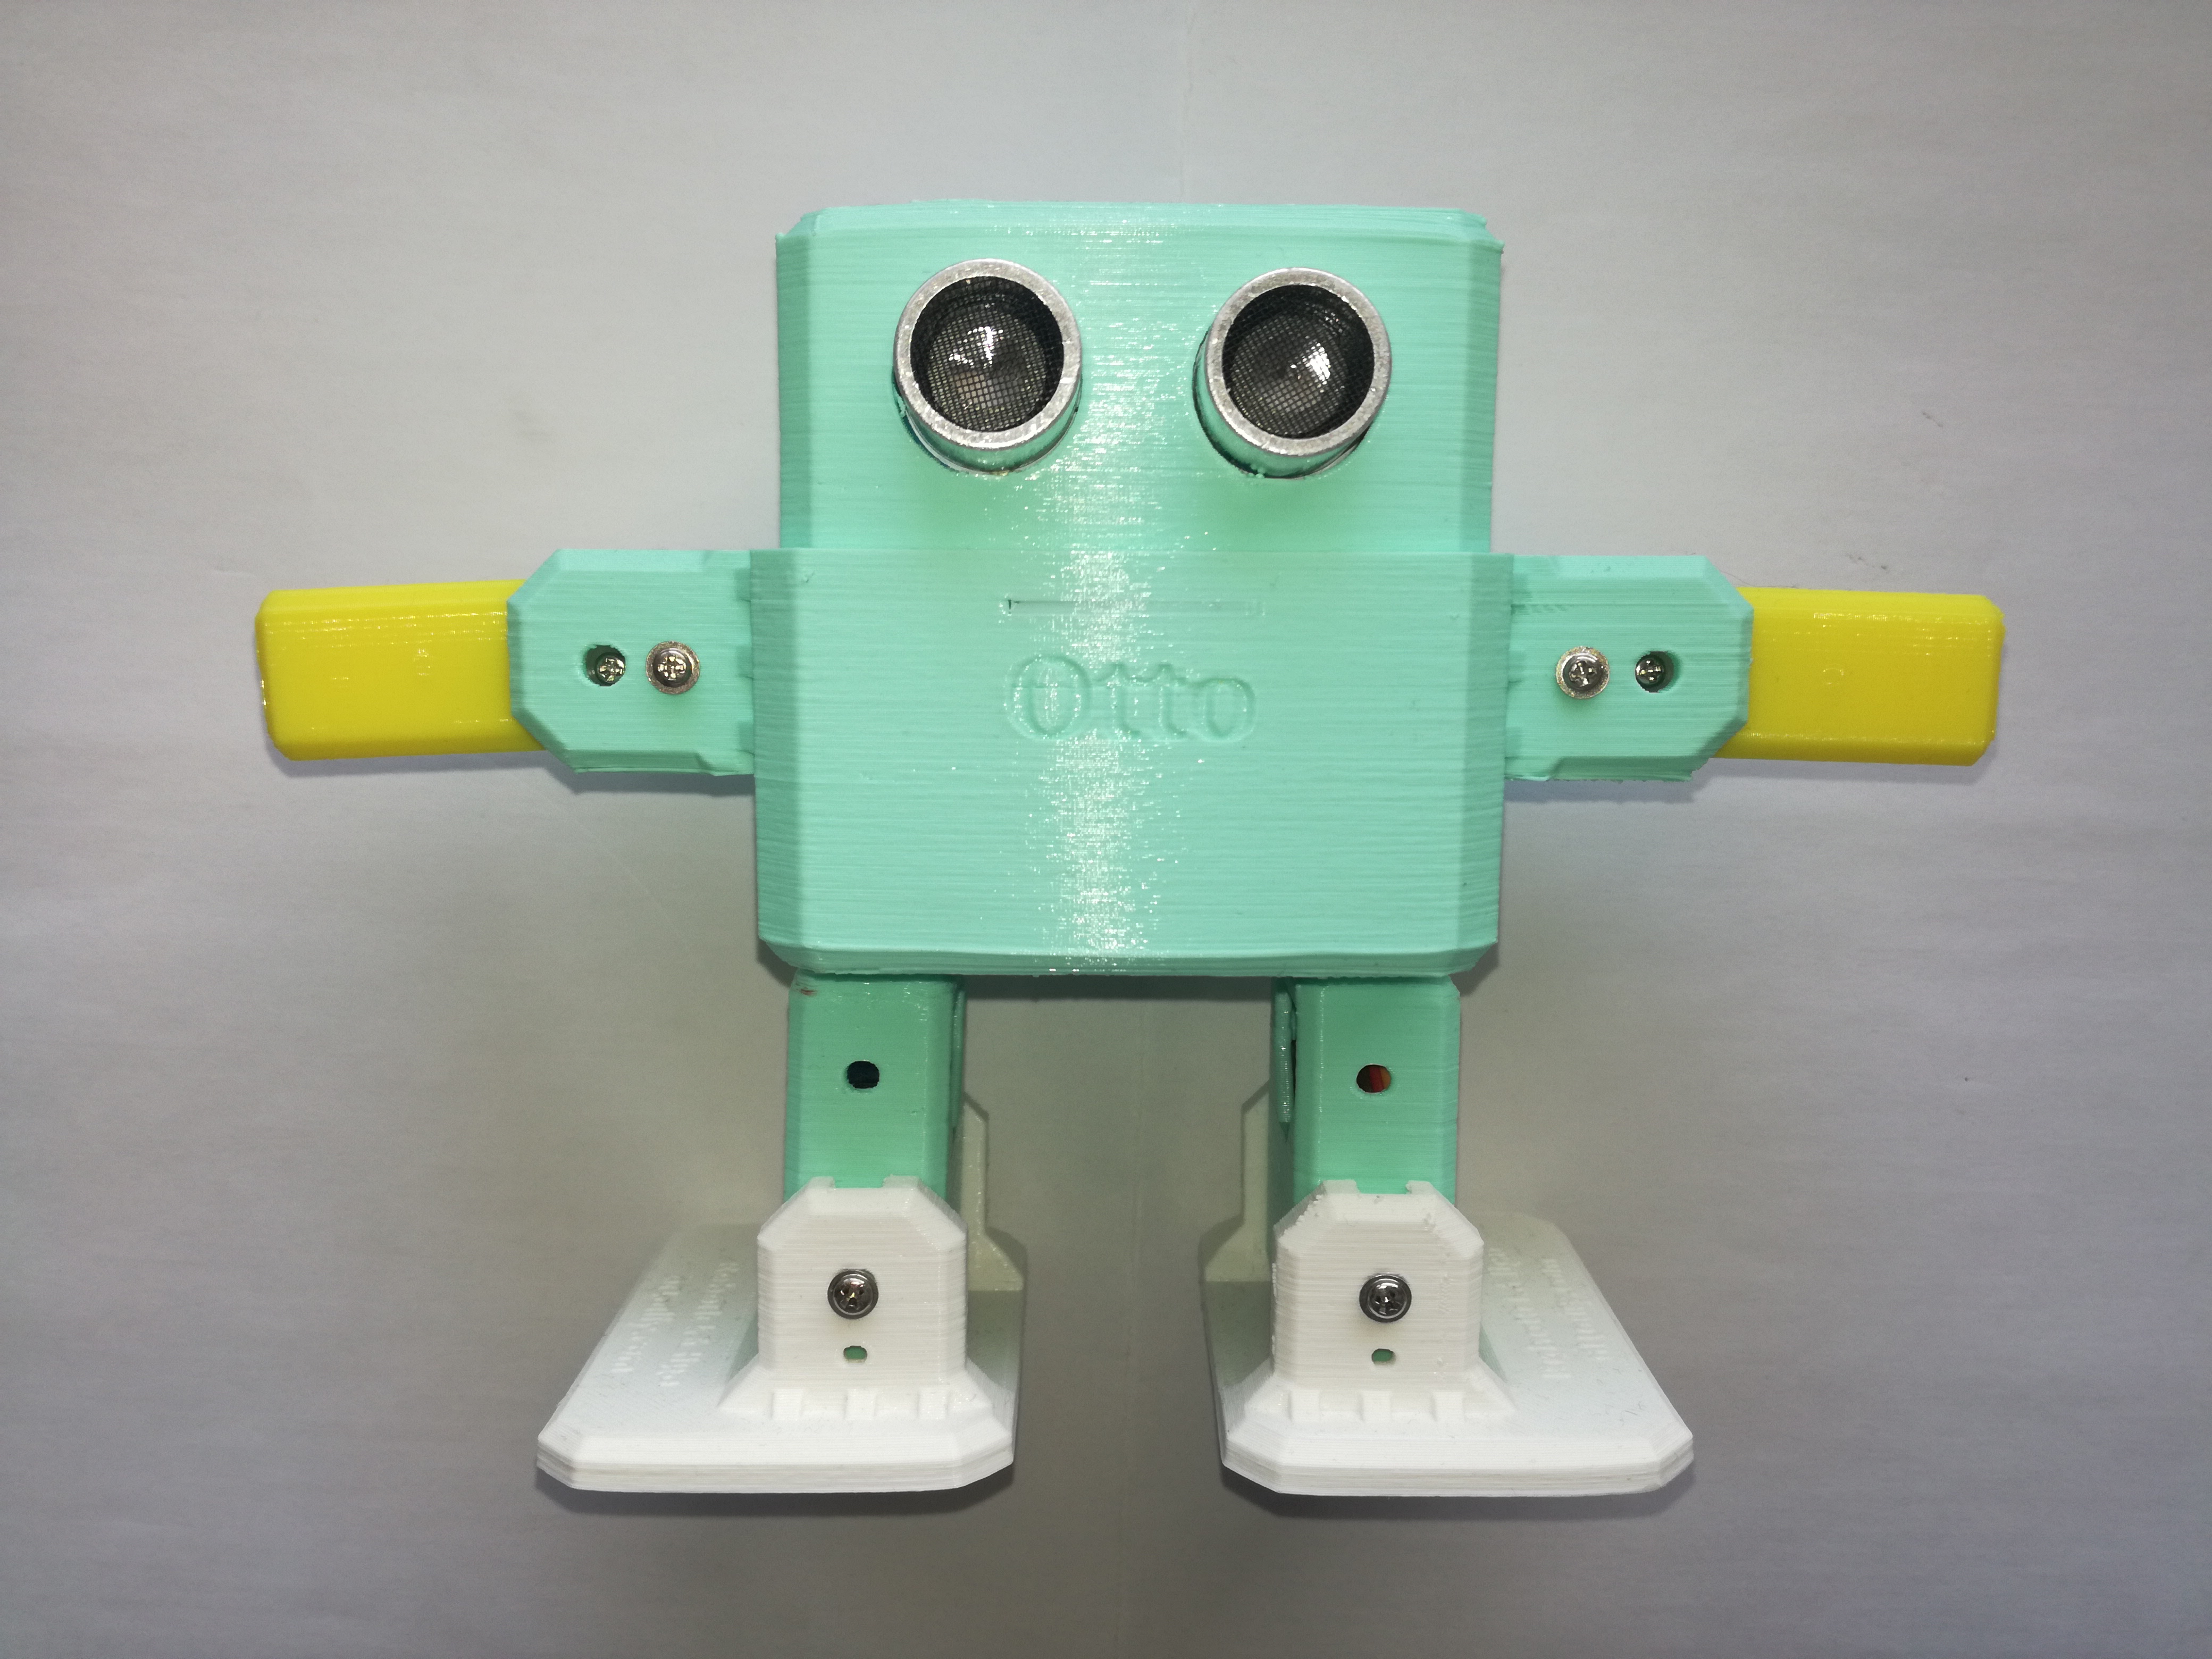
\includegraphics[width=0.4\textwidth]{images/otto}}
\caption[Robot Otto]{Robot Otto}
\label{obr:otto}
\end{figure}

\subsubsection{Riadiaci program, interakcia, programovanie}
Program vykonávaný Arduinom nie je prebraný od vynálezcov pôvodnej verzie robota. Vytvoril ho špeciálne pre účely denného tábora školiteľ tejto práce, Mgr. Pavel Petrovič, PhD. V najnovšej verzii (21.11.2018) sú v zásade možné dva varianty interakcie s robotom. Možno ho ovládať priamo, teda robot vykonáva príkazy prijaté cez sériový port ihneď. Takéto povely sú charakteru \uv{posuň motor A dopredu} alebo \uv{pípni}. Druhým prístupom je programovanie. Jedným z interpretovaných znakov --- príkazov je aj špeciálny znak na prechod do režimu programovania. Tu je možné zadať program ako postupnosť trojíc (doba čakania v milisekundách, číslo motora, rotácia motora v stupňoch) a niekoľkých špeciálnych príkazov (tiež ako trojice), ktoré umožňujú napríklad \uv{skoky} v programe (v podstate inštrukcia jump --- vykonávanie programu pokračuje zadaným riadkom kódu, za čo sa považuje každá takáto trojica). Súčasťou sú tiež trojice --- inštrukcie na prehranie melódie, prípadne zvukového efektu. Takto vytvorený program je ukladaný do pamäte RAM, v riadiacom programe vykonávanom v mikropočítači sú spomínané trojice reprezentované ako prvky poľa celých čísel. Programovanie je teda značne limitované veľkosťou pamäte, nie je prehľadné, a nakoľko program nemožno editovať, často nie je ani praktické. Výhodou však stále bezpochyby zostáva možnosť interakcie a tvorby choreografie bez znalosti C++.

% Mokrarosa
\subsection{Robot Mokrarosa}
Robot MoKraRosA (MOdulárny KRAhulský RObot S Arduinom) bol témou Denného tábora digitálnych technológií v roku 2019. Vyvinutý je od základu v dielni Fablab Bratislava kde bolo toho roku skonštruovaných 80 kusov s podobným cieľom ako predtým robot Otto \cite{Mokrarosa}.

\subsubsection{Konštrukcia, možnosti, schopnosti}
Telo robota Mokrarosa pripomína pavúka, aj keď má len štyri nohy. Aj tu bol použitý rovnaký modul pre senzor merania vzdialenosti od prekážky ktorý v dizajne imituje \uv{oči} prístroja. Pavúk je navyše osadený gyroskopom, ktorý mu umožňuje reagovať na preklopenie, prípadne pád. Konštrukcia dovoľuje nohami robota prevrátiť alebo vykonať kotúľ, pričom na základe údajov z gyroskopu môže vždy nasmerovať' nohy smerom k zemi a tak sa nikdy nedostane do polohy, z ktorej by nebol možný pohyb (na rozdiel od robota Otto). Štandardne je tiež osadený dvoma výstupnými zariadeniami, mp3 prehrávačom a reproduktorom.

TODO: obrazok Mokrarosa

\subsubsection{Riadiaci program, interakcia, programovanie}
Riadiaci program pavúka je o niečo zložitejší. Umožňuje jednak robota riadiť \uv{po znakoch}, v tomto móde ihneď reaguje na symbol prijatý cez sériový port, obdobne ako v prípade robota Otto. V režime programovania sa výraznejšie líši. Program je daný ako postupnosť n-tíc kde každá n-tica vyjadruje v akej polohe (v stupňoch) sa má v daný moment daný motor nachádzať. Je tak možné hýbať s viacerými motormi naraz. Podstatný rozdiel je tiež v postupe programovania. Program je možné tvoriť tak, že robota postupne navádzame v režime \uv{po znakoch}, teda manuálnym pohybom jednotlivými motormi, do požadovanej polohy a následne uložíme stav --- natočenie každého z motorov do spomínanej n-tice. Takto postupne vytvárame \uv{pózy}, cez ktoré robot následne plynule prechádza.


% ===
% === Existujúce riešenia
% ===
\section{Existujúce riešenia}
Jediné nám známe dostupné príbuzné riešenie, v súvislosti s robotmi Otto a Mokrarosa, pochádza priamo od tvorcov robota Otto, ktorí vyvinuli pomerne rozsiahlu aplikáciu na tvorbu jeho riadiacich programov. V prípade robota Mokrarosa podobné riešenia pochopiteľne neexistujú, nakoľko je len nedávnym produktom dielne Fablab Bratislava. Uvádzame však i iné riešenia súvisiace s výučbou robotiky a programovania.

\subsection{Otto Blockly}
Ide o desktopovú aplikáciu umožňujúcu programovať robota Otto v grafickom jazyku, vytvorenom pomocou knižnice Google Blockly \cite{OttoBlockly}. Produktom sa možno vo viacerých aspektoch inšpirovať. Aplikácia je profesionálne graficky spracovaná, podporuje rôzne funkcie robota, ponúka okamžitý preklad vytvoreného kódu riadiaceho programu do C++, ktorý možno ľahko kompilovať a nahrať priamo do pripojeného mikropočítača Arduino.

Nevýhodou pre nás je predovšetkým naviazanosť na robota z výroby autorov. Nami používaný klon robota Otto je modifikovaný a tak by pre použitie s aplikáciou bolo potrebné s každou zmenou zapojenia zmeniť aj logiku generátora kódu v aplikácii. Rovnako aplikácia nepodporuje štýl programovania kde sú vytvárané choreografie ukladané bez potreby kompilácie do pamäte RAM. Tento prístup je pritom mimoriadne výhodný pri častom ladení jednoduchých choreografii. 

\subsection{Lego Mindstorms}
TODO ( + alternatívy k mindstorms sw)

\subsection{CodeSnaps}
TODO, možno presun do sekcie "možné rozšírenia"
